%%==================================================
%% demo.tex for BIT Master Thesis
%% modified by yang yating
%% version: 0.5
%% last update: April 25th, 2017
%%==================================================

\documentclass[oneside, master]{BIT-thesis-grd}

\begin{document}

%%%%%%%%%%%%%%%%%%%%%%%%%%%%%%
%% 封面
%%%%%%%%%%%%%%%%%%%%%%%%%%%%%%

% 中文封面内容(关注内容而不是形式)
\title{BIT-Thesis使用指南\\ v1.0}
\author{北京理工大学~~研究生院}
\defenddate{2017年9月}

% 封面,这个命令实现了形式,具体见.cls
\maketitle

%%%%%%%%%%%%%%%%%%%%%%%%%%%%%%
%% 前言
%%%%%%%%%%%%%%%%%%%%%%%%%%%%%%
\frontmatter

% 目录
\tableofcontents
% 表格索引
%\listoftables
% 插图索引
%\listoffigures

%\addcontentsline{toc}{chapter}{\listfigurename} %将表格索引加入全文目录
%\addcontentsline{toc}{chapter}{\listtablename}  %将图索引加入全文目录

% 主要符号、缩略词对照表
% \include{body/symbol}

%%%%%%%%%%%%%%%%%%%%%%%%%%%%%%
%% 正文
%%%%%%%%%%%%%%%%%%%%%%%%%%%%%%
\mainmatter  %处理正文编号

%% 各章正文内容
%%==================================================
%% ch1.tex for BIT Master Thesis
%% modified by yang yating
%% version: 0.2
%% last update: March 30th, 2017
%%==================================================

\chapter{快速使用指南}
\label{chap:what}

本手册是针对北京理工大学硕士(博士)学位论文~\LaTeX~ 模板BIT-thesis的使用指南。旨在使同学们通过该使用指南的介绍,能快速使用BIT-thesis模板编辑符合学校格式要求的硕士(博士)学位论文,并能对~\LaTeX~ 有一定的了解。

\section{为什么要用BIT-Thesis}
\label{sec:why}
学位论文通常具有比较严格的格式要求,这是为了方便同行学术交流的起码要求,同时也是科学研究严谨性的体现。然而,由于市场各种排版软件混杂,使用者水平不一,学生对格式的重视程度不够,学生编写标准格式的学位论存在很多问题。BIT-Thesis 为符合北京理工大学硕士(博士)学位论文的LaTex模板。通过BIT-Thesis模板可以轻松攥写符合学校格式要求的学位论文,学生可将关注点更多地放在高质量的内容本身,而避免繁琐的论文格式调整。

\section{安装配置环境}
\label{sec:requirements}

为了安装便捷,推荐安装Ctex套装。

\begin{itemize}
\item \textit{Ctex套装下载地址}  http://www.ctex.org/CTeXDownload

\item \textbf{或者使用北京理工大学开源软件镜像服务}  http://mirror.bit.edu.cn/CTAN

\end{itemize}



\section{快速使用}
\label{sec:process}

安装完ctex套装后,一般而言所需的环境就配置好了。

下面以硕士学位论文模板\textbf{BIT-thesis-template-master}为例,进入BIT-thesis-template-master文件夹。
windows系统点击运行BIT-thesis-run.bat脚本,linux系统以及mac系统请点击运行BIT-thesis-run.sh脚本。脚本会自动运行如图\ref{fig:run} 所示(第一次运行可能需要较长时间,请耐心等待)。打开生成的pdf文档demo.pdf查看模板生成内容。
 
\begin{figure}[!htp]
  \centering
  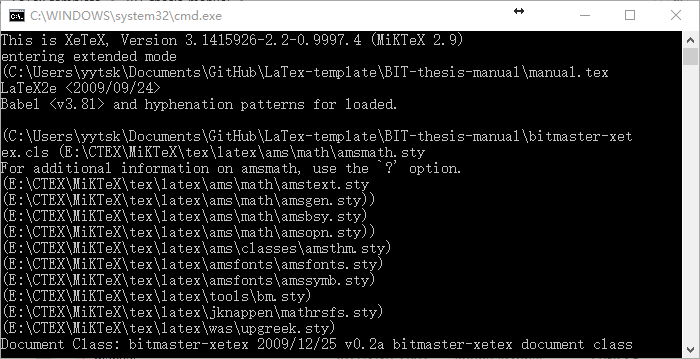
\includegraphics[width=0.8\textwidth]{figures/BIT-thesis-run}
  \caption{BIT-thesis-run.bat脚本运行}
  \label{fig:run}
\end{figure}


\begin{figure}[!htp]
  \centering
  {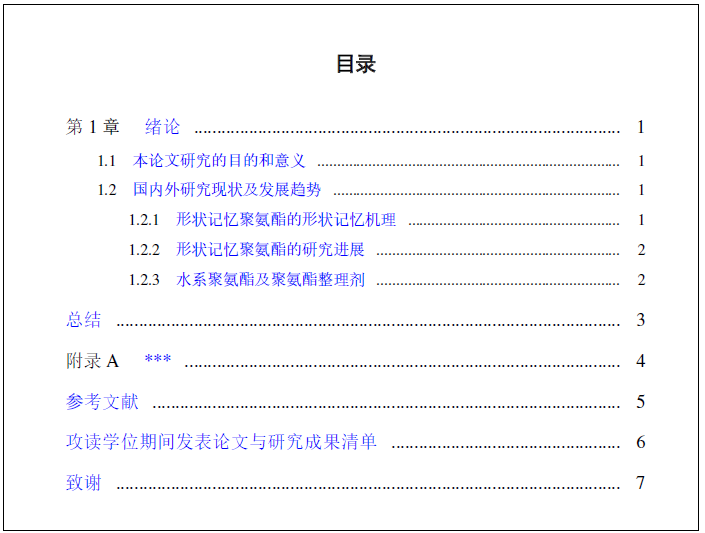
\includegraphics[width=0.8\textwidth]{figures/demo_context}}
  \caption{生成文档demo.pdf的目录}
  \label{fig:demo_context}
\end{figure}

本模板使用~\XeTeX~ 引擎提供的~xelatex~的命令处理,作用于“主控文档”demo.tex。
并且,可以省略扩展名。完整的处理流程是:

{\color{blue}
\begin{enumerate}
\item[] ~\verb|xelatex -no-pdf --interaction=nonstopmode demo|
\item[] ~\verb|bibtex demo| 
\item[] ~\verb|xelatex -no-pdf --interaction=nonstopmode demo|
\item[] ~\verb|xelatex --interaction=nonstopmode demo|
\end{enumerate}}

运行bibtex的时候会提示一些错误,可能是~{{\sc Bib}\TeX}~对UTF-8支持不充
分,一般不影响最终结果。加入~\verb|--interaction=nonstopmode|~参数是不让错误打断编译过程。
\XeTeX~ 仍存在一些宏包兼容性问题,而这些错误通常不会影响最终的编译结果。
  
为方便使用,处理过程已经写入BIT-thesis-run.sh(for Linux)和BIT-thesis-run.bat(for Windows)批处理文件中。编写完修改完tex文件后,直接运行对应.sh或者.bat文件即可。


\section{模板说明与Tex介绍}
\label{sec:features}
 
目前网上有两个版本的北理工~\LaTeX~ 模板“2012大眼小蚂蚁版”和“2016汪卫版”,均以上海交通大学的模为基础。本模板在此两个模板的基础上依据《北京理工大学博士、硕士学位论文撰写规范》修改,进一步完善成熟,使得模板能够被北理工硕士博士广泛使用。希望使用者通过本模板的介绍对~\LaTeX~ 有一定了解。

这个模板的中文解决方案是~\XeTeX/\LaTeX~ 。参考
文献建议使用~BibTeX~管理,可以生成符合国标~GBT7714~风格的参考文献列表。
可以直接插入EPS/PDF/JPG/PNG格式的图像。
模板在~Windows~和~Linux~下测试通过,更详细的系统要求请参考
\ref{sec:requirements}。

硕士模板的格式受~bitmater-xetex.cls~和~bitmaster-xetex.cfg~控制,博士模板的格式受~bitdoctor-xetex.cls~和~bitdoctor-xetex.cfg~控制方便模板更新和模板修改。依据《北京理工大学博士、硕士学位论文撰写规范》修改,按照本文档说明使用,即可撰写符合《北京理工大学博士、硕士学位论文撰写规范》的学位论文;
在对外观进行细微调整时,只需要更新这两个文件,不需要对.tex源文件做修改。这也给模板更新带来了
极大方便。\textbf{一般使用者不需要修改这两个文件。}
 
~XeLaTeX~ 对应的XeTeX对中文字体的支持更好,允许用户使用操作系统字体来代替TeX的标准字体。所以本模板使用~XeLaTeX~ 引擎处理中文。要使用这个模板协助你完成研究生学位论文的创作,下面的条件必须满足:

\begin{itemize}
\item \inv 操作系统字体目录中有中文字体(adobe或windows字体均可);
\item \inv \TeX~系统有~\XeTeX~引擎;
\item \inv \TeX~系统有~ctex~宏包;
\item \inv \TeX~系统的fontspec宏包(fontspec.sty)足够新;
\item \inv 你有使用~\LaTeX~的经验。
\end{itemize}

安装完成后,便可对tex进行编写以生成相应论文,也可更具使用习惯使用texmaker、Winedit等其他的编辑器进行编写(推荐使用texmaker)。




%%==================================================
%% ch2.tex for BIT Master Thesis
%% modified by yang yating
%% version: 0.5
%% last update: April 25th, 2017
%%==================================================

\chapter{模板使用}
\label{chap:textStructure}

本章的目的是介绍\LaTeX{}的文本控制流程,即如何实现学位论文在各章节中的分布,以及章节内的交叉引用问题,用户可以根据自身对\LaTeX{}的熟悉程度适当地略过阅读。在了解了本章的内容后,用户即可通过文本内容的粘贴和复制,快速实现生成一个格式满足基本需求的文档。

以硕士模板为例,文件布局如图\ref{layout-master}所示。

\begin{lstlisting}[basicstyle=\small\ttfamily,caption={BIT-thesis-template-master 模板文件布局},label=layout-master,numbers=none]
  ├── demo.tex              主控文件
  ├── demo.pdf              生成的论文pdf
  ├── bitmaster-xetex.cfg   格式控制文件(布局设置文件)
  ├── bitmaster-xetex.cls   格式控制文件(文档类文件)
  ├── GBT7714-2005NLang.bst 参考文献格式控制文件
  ├── chapters              章节文件夹
  │   ├── abstract.tex       摘要
  │   ├── chapter01.tex      第一章
  │   ├── conclusion.tex     总结
  │   ├── app1.tex           附录A
  │   ├── pub.tex            攻读学位期间发表论文与研究成果清单
  │   └── thanks.tex         致谢
  ├── figures               图片文件夹
  │   └── figure1.png   
  ├── reference             参考文献文件夹
  │   └── chap1.bib
  ├── BIT-thesis-run.cmd    运行脚步cmd
  └── BIT-thesis-run.sh     运行脚本sh
  
      
\end{lstlisting}

\section{认识模板组成}

\subsection{格式控制文件}
\label{sec:format}

格式控制文件控制着论文的表现形式,包括以下几个文件:
bitmaster-xetex.cfg, bitmaster-xetex.cls~和~GBT7714-2005NLang.bst。
其中,``.cfg''和``.cls''控制论文主体格式,``.bst''控制参考文献条目的格式,

一般用户可以``忽略''格式控制文件的存在。因为该文件已经按照《北京理工大学博士、硕士学位
论文撰写规范》进行了修改。有其他格式修改的需要,参见第\ref{sec:thesisformat}章。


\subsection{主控文件~demo.tex}
\label{sec:demotex}

主控文件~demo.tex~的作用就是将分散在多个文件中的内容``整合''成一篇完整的论文。
使用这个模板撰写学位论文时,学位论文内容和素材会被``拆散''到各个文件中:
譬如各章正文、各个附录、各章参考文献等等。
在~demo.tex~中通过``include''命令将论文的各个部分包含进来,从而形成一篇结构完成的论文。
封面页中的论文标题、作者等中英文信息,也是在~demo.tex~中填写。也可以在demo.tex中按照自己的需要引入一些的宏包
\footnote{一般只有当你需要在文档中使用那个宏包时,才需要在导言区中用~usepackage~引入该宏包。如若不然,通过usepackage引入一大堆不被用到的宏包,必然是一场灾难。由于一开始没有一致的设计目标,\LaTeX~ 的各宏包几乎都是独立发展起来的,因重定义命令导致的宏包冲突屡见不鲜。}。

大致而言,在主控文件~demo.tex~中,只需要留意文章有哪些章节以及各章参考文
献内容,不需要具体关注每一章里面的具体内容。需要注意,处理文档时所有的操作命令
{}\cndash{}xelatex, bibtex等,都是作用在~demo.tex~上,而\emph{不是}后面这
些``分散''的文件,请参考\ref{sec:process}小节。


\subsection{论文主体文件夹chapters}
\label{sec:thesisbody}

这一部分是论文的主体,是以``章''为单位划分的。

正文前部分(frontmatter):中英文摘要(abstract.tex)。其他部分,诸如中英文封
面、授权信息等,都是根据~demo.tex~所填的信息``画''好了,不单独弄成文件。

正文部分(mainmatter):是各章内容,在chapter文件夹中。

正文后的部分(backmatter):附录(app\emph{xx}.tex);致谢(thuanks.tex);攻读
学位论文期间发表的学术论文目录(pub.tex);作者简介(resume.tex)。参考文献列
表是``生成''的,也不作为一个单独的文件。另外,学校的硕士研究生学位论文模
板没有要求加入作者简介,但博士的学位论文要求加入作者简介。


\subsection{图片文件夹~figures}
\label{sec:figuresdir}

figures~文件夹放置了需要插入文档中的图片文件(PNG/JPG/PDF/EPS)。如果图片较多,建议按章再
划分子目录存储图片。

\subsection{参考文献数据库文件夹~reference}
\label{sec:bibdir}

reference~文件夹放置的是各章``可能''会被引用的参考文献文件。参考文献的元
数据,例如作者、文献名称、年限、出版地等,会以一定的格式记录在纯文本文
件.bib中。最终的参考文献列表是BibTeX处理.bib后得到的,名为~demo.bbl。将参
考文献按章划分的一个好处是,可以在各章后生成独立的参考文献,不过,现在看
来没有这个必要。关于参考文献的管理,可以进一步参考第\ref{chap:example}章
中的例子。


\section{进行论文写作}
\label{sec:format}

本节介绍使用论文模板,修改论文信息、摘要、关键字,以及编辑章节等。

\subsection{封面和标题}
在主控文件demo.tex中填写论文的相应信息。

中文封面信息:
\begin{itemize}
\item 中图分类号(\verb|\classification{TQ028.1}|)
\item UDC分类号(\verb|\UDC{540}|)
\item 论文标题(\verb|\title{论文标题}|)
\item 作者姓名(\verb|\author{姓名}|)
\item 学院名称(\verb|\institute{学院名称}|)
\item 指导教师(\verb|\advisor{教授姓名}|)
\item 答辩委员会主席(\verb|\chairman{教授姓名}|)
\item 申请学位(\verb|\degree{学位名称}|)
\item 学科专业(\verb|\major{专业名称}|)
\item 学位授予单位(\verb|\school{北京理工大学}|)
\item 论文答辩日期(\verb|\defenddate{答辩日期}|)
\end{itemize}


英语封面信息:
\begin{itemize}
\item English Title(\verb|\englishtitle{论文标题}|)
\item Candidate Name(\verb|\englishauthor{姓名}|)
\item School or Department(\verb|\englishinstitute{学院名称}|)
\item Faculty Mentor(\verb|\englishadvisor{教授姓名}|)
\item Chair,Thesis Committee(\verb|\englishchairman{教授姓名}|)
\item Degree Applied(\verb|\englishdegree{学位名称}|)
\item Major(\verb|\englishmajor{专业名称}|)
\item Degree by(\verb|\englishschool{Beijing Insititute of Technology}|)
\item The Data of Defence(\verb|\englishdate{答辩日期}|)
\end{itemize}

\subsection{摘要和关键字}
摘要内容,放置于chapters文件夹下的abstract.tex中,

中文摘要于\verb|abstract|环境编写;\verb|\keywords|为中文关键字。英文摘要于\verb|englishabstract|环境编写;\verb|\englishkeywords|为中文关键字。

\begin{lstlisting}[language={[LaTeX]TeX}, caption={中英文摘要}]
\begin{abstract}
	本文 ...
\keywords { 形状记忆;聚氨酯 }
\end{abstract}

\begin{englishabstract}
   In order to exploit ...
\englishkeywords{shape memory properties; polyurethane}
\end{englishabstract}
\end{lstlisting}


\subsection{正文章节}
章节的设置分别通过关键字完成,按照章节的级别依此如表~\ref{tab:setSection}所示,关于文档中具体章节的关键词设置可以参看原宏包中tex文件夹下的实例文件。

\begin{table}[htb]
 \centering
  \caption{章节设置关键字}     % title of Table
  \label{tab:setSection}    % label of Table
  \begin{tabular}{cl}
    \hline
    章节级别        & 关键字     \\
    \hline
     章        & \verb|\chapter| \\
     节        & \verb|\section | \\
    子节      & \verb|\subsection |\\
    表格名称       & \verb|\caption{章节设置关键字}| \\
    引用标签       & \verb|\label{sec:labelName}| \\
    \hline
  \end{tabular}
\end{table}

\subsection{其他部分}


全文总结、攻读学位期间发表论文与研究成果清单、致谢的内容,均位于chapters文件夹下,分别为conclusion.tex,pub.tex,thanks.tex。

\section{交叉引用}
\subsection{公式、图表和插图引用}
\label{sec:refofFigAndTab}
交叉引用的前提是需要在定义章节、公式和图表的时候都对其进行命名标签(即\textbackslash label\{sec:labelName\}命令),在实际使用过程中通过标签进行引用。根据引用的特点可以将应用分成表~\ref{tab:citeType}中所示三类。

\begin{table}[htb]
 \centering
  \caption{交叉引用类型}       % title of Table
  \label{tab:citeType}    % label of Table
  \begin{tabular}{cl}
    \hline
    引用类型     & 关键字     \\
    \hline
    标签设置        & \textbackslash label\{marker\}  \\
    引用代号        & \textbackslash ref\{marker\}    \\
    引用页码        & \textbackslash pageref\{marker\} \\
    引用文献        & \textbackslash cite\{regLabel\} \\
    \hline
  \end{tabular}
\end{table}

其中,表格和图片的摆放位置由 \textbackslash begin\{table\}或\textbackslash begin\{figure\}后面的中括号设置,例如[htb]表示可以将图表放在当前位置(here)、页面顶端(top)或者页面底端(bottom)。

{\bf{实例1:}}这里是对表格《交叉引用类型》的引用——表~\ref{tab:citeType}位于第~\pageref{tab:citeType}页,其标签为\textbackslash label\{tab:citeType\}。


\subsection{文献引用}
\label{sec:citeRefs}

BIT-Thesis论文模板使用BibTeX处理参考文献。

参考文献的具体内容就是reference文件夹下的chap\textit{xx}.bib,参考文献的元数据(名称、作者、出处等)以一定的格式保存在这些纯文本文件中。
.bib文件也可以理解为参考文献的``数据库'',正文中所有引用的参考文件条目都会从这些文件中``析出''。

正文中引用参考文献时,用\verb+\upcite{...}+可以产生“上标引用的参考文献”,
如\upcite{chen2007act},\upcite{Meta_CN,chen2007act,DPMG}。

具体使用方法参见第\ref{sec:reference}节。

%%==================================================
%% ch3.tex for BIT Master Thesis
%% modified by yang yating
%% version: 0.2
%% last update: Feb 16th, 2017
%%==================================================


% \bibliographystyle{bit2} %[此处用于每章都生产参考文献]
\chapter{公式、图像和表格}
\label{chap:example}
公式、图表和插图广泛使用于学位论文中,并且在正文内存在较多的交叉引用,对他们的高效处理也是\LaTeX{}的优势之一。公式、图表和插图在定义时的共同特点包含:定义中需要设定引用标签、设置图表名称。定义时,图表摆放位置并无要求,\LaTeX{}会根据文稿内容自动计算图表摆放位置,不会出现表格窜行的问题。

\section{公式与数学环境}
\label{sec:eqn}

\subsection{公式及术语表}
\label{sec:eqn}

公式定义的内容包含在\verb|\begin{equation}|\verb|\end{equation}|之间。为方便,公式的编辑可以采用在线的\LaTeX{}公式编辑器。公式的编号格式可以在./sty文件夹下的格式文件中定义,公式中涉及的术语表也需要在公式后面进行对应标记。一般的\LaTeX{}编辑器如Winedit、texmaker等都有公式编辑器。

{\bf{实例1:}} 以下是L-B非稳态流动升力模型,公式引用为公式\ref{eqn:LBmodel}。该公式的术语列表见 表 \ref{tab:LB-parameters}。
\begin{equation}
 \label{eqn:LBmodel}
   C_{L}=C_{L0}+C_{L\alpha }\left ( \frac{1+\sqrt{X}}{2} \right )\alpha 
\end{equation}

\begin{lstlisting}[language={TeX}, caption={L-B非稳态流动升力模型}]
\begin{equation}
 \label{eqn:LBmodel}
   C_{L}=C_{L0}+C_{L\alpha }\left ( \frac{1+\sqrt{X}}{2} \right )\alpha 
\end{equation}
\end{lstlisting}

\subsection{长公式排版}


《Math mode》里有举一个长公式排版的例子如下。《Math mode》有十分丰富实用的例子,感兴趣的同学可以参考一下。

\begin {multline}
  \frac {1}{2}\Delta (f_{ij}f^{ij})=
  2\left (\sum _{i<j}\chi _{ij}(\sigma _{i}-
    \sigma _{j}) ^{2}+ f^{ij}\nabla _{j}\nabla _{i}(\Delta f)+\right .\\
  \left .+\nabla _{k}f_{ij}\nabla ^{k}f^{ij}+
    f^{ij}f^{k}\left [2\nabla _{i}R_{jk}-
      \nabla _{k}R_{ij}\right ]\vphantom {\sum _{i<j}}\right )
\end{multline}

\begin{lstlisting}[language={TeX}, caption={长公式排版}]
\begin {multline}
  \frac {1}{2}\Delta (f_{ij}f^{ij})=
  2\left (\sum _{i<j}\chi _{ij}(\sigma _{i}-
    \sigma _{j}) ^{2}+ f^{ij}\nabla _{j}\nabla _{i}(\Delta f)+\right .\\
  \left .+\nabla _{k}f_{ij}\nabla ^{k}f^{ij}+
    f^{ij}f^{k}\left [2\nabla _{i}R_{jk}-
      \nabla _{k}R_{ij}\right ]\vphantom {\sum _{i<j}}\right )
\end{multline}
\end{lstlisting}

\subsection{定理环境}

在~bitmaster-xetex.cfg~中定义了丰富的定理环境
algo(算法),thm(定理),lem(引理),prop(命题),cor(推论),defn(定义),conj(猜想),exmp(例),rem(注),case(情形),
bthm(断言定理),blem(断言引理),bprop(断言命题),bcor(断言推论)。
amsmath还提供了一个proof(证明)的环境。
这里举一个``定理''和``证明''的例子。
\begin{thm}[留数定理]
\label{thm:res}
  假设$U$是复平面上的一个单连通开子集,$a_1,\ldots,a_n$是复平面上有限个点,$f$是定义在$U\backslash \{a_1,\ldots,a_n\}$上的全纯函数,
  如果$\gamma$是一条把$a_1,\ldots,a_n$包围起来的可求长曲线,但不经过任何一个$a_k$,并且其起点与终点重合,那么:

  \begin{equation}
    \label{eq:res}
    \ointop_{\gamma}f(z)\,\mathrm{d}z = 2\uppi\mathbf{i}\sum^n_{k=1}\mathrm{I}(\gamma,a_k)\mathrm{Res}(f,a_k)
  \end{equation}

  如果$\gamma$是若尔当曲线,那么$\mathrm{I}(\gamma, a_k)=1$,因此:

  \begin{equation}
    \label{eq:resthm}
    \ointop_{\gamma}f(z)\,\mathrm{d}z = 2\uppi\mathbf{i}\sum^n_{k=1}\mathrm{Res}(f,a_k)
  \end{equation}

      % \oint_\gamma f(z)\, dz = 2\pi i \sum_{k=1}^n \mathrm{Res}(f, a_k ). 

  在这里,$\mathrm{Res}(f, a_k)$表示$f$在点$a_k$的留数,$\mathrm{I}(\gamma,a_k)$表示$\gamma$关于点$a_k$的卷绕数。
  卷绕数是一个整数,它描述了曲线$\gamma$绕过点$a_k$的次数。如果$\gamma$依逆时针方向绕着$a_k$移动,卷绕数就是一个正数,
  如果$\gamma$根本不绕过$a_k$,卷绕数就是零。

  定理\ref{thm:res}的证明。
  
  \begin{proof}
    首先,由……

    其次,……

    所以……
  \end{proof}
  
\end{thm}

上面的公式例子中,有一些细节需要注意。微分号d应该使用``直立体'',也就是用mathrm包围起来。
并且,微分号和被积函数之间应该有一段小间隔,可以插入\verb+\,+得到。
斜体的$d$通常只作为一般变量。
i,j作为虚数单位时,也应该使用``直立体'',为了明显,还加上了粗体,例如\verb+\mathbf{i}+。斜体$i,j$通常用作表示``序号''。
其他字母在表示常量时,也推荐使用``直立体'',譬如,圆周率$\uppi$(需要upgreek宏包),自然对数的底$\mathrm{e}$。


\section{向文档中插入图像}
\label{sec:insertimage}

\subsection{支持的图片格式}
\label{sec:imageformat}

\XeTeX~ 可以很方便地插入~PDF、EPS、PNG、JPG~格式的图片。在学位论文中,插图地使用简单地分为两类:单列图片和多列图片。图片地格式包含*.jpg、*.eps、*.pdf,既可以是位图也可以是矢量图,在插入图片是可以定义其高度和宽度。

插入PNG/JPG的例子如\ref{fig:SRR}所示。
这两个水平并列放置的图共享一个``图标题''(table caption),没有各自的小标题。

\begin{figure}[!htp]
  \centering
  
\includegraphics[width=0.3\textwidth]{figures/BIT}
  \hspace{1cm}
  
\includegraphics[width=0.3\textwidth]{figures/BIT-CS}
  \caption{校徽以及计算机学院LOGO}
\end{figure}

\begin{lstlisting}[language={TeX}, caption={插入PNG/JPG}]
\begin{figure}[!htp]
  \centering
  
\includegraphics[width=0.3\textwidth]{figures/BIT}
  \hspace{1cm}
  
\includegraphics[width=0.3\textwidth]{figures/BIT-CS}
  \caption{校徽以及计算机学院LOGO}
\end{figure}
\end{lstlisting}

这里还有插入eps图像和pdf图像的例子,如图\ref{fig:pdfeps}。这里将EPS和PDF图片作为子图插入,每个子图有自己的小标题。并列子图的功能是使用~subfigure~宏包提供的。

\begin{figure}
  \centering
  \subfigure[EPS Figure]{
    \label{fig:epspdf:a} %% label for first subfigure
    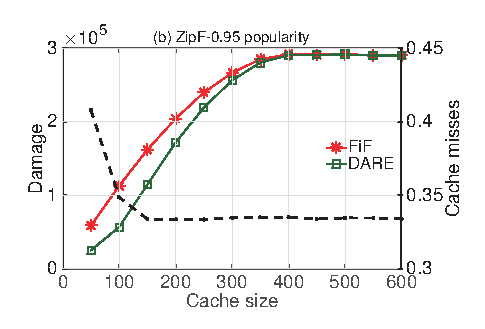
\includegraphics[width=0.45\textwidth]{figures/pic-eps}}
  \subfigure[PDF Figure]{
    \label{fig:epspdf:b} %% label for second subfigure
    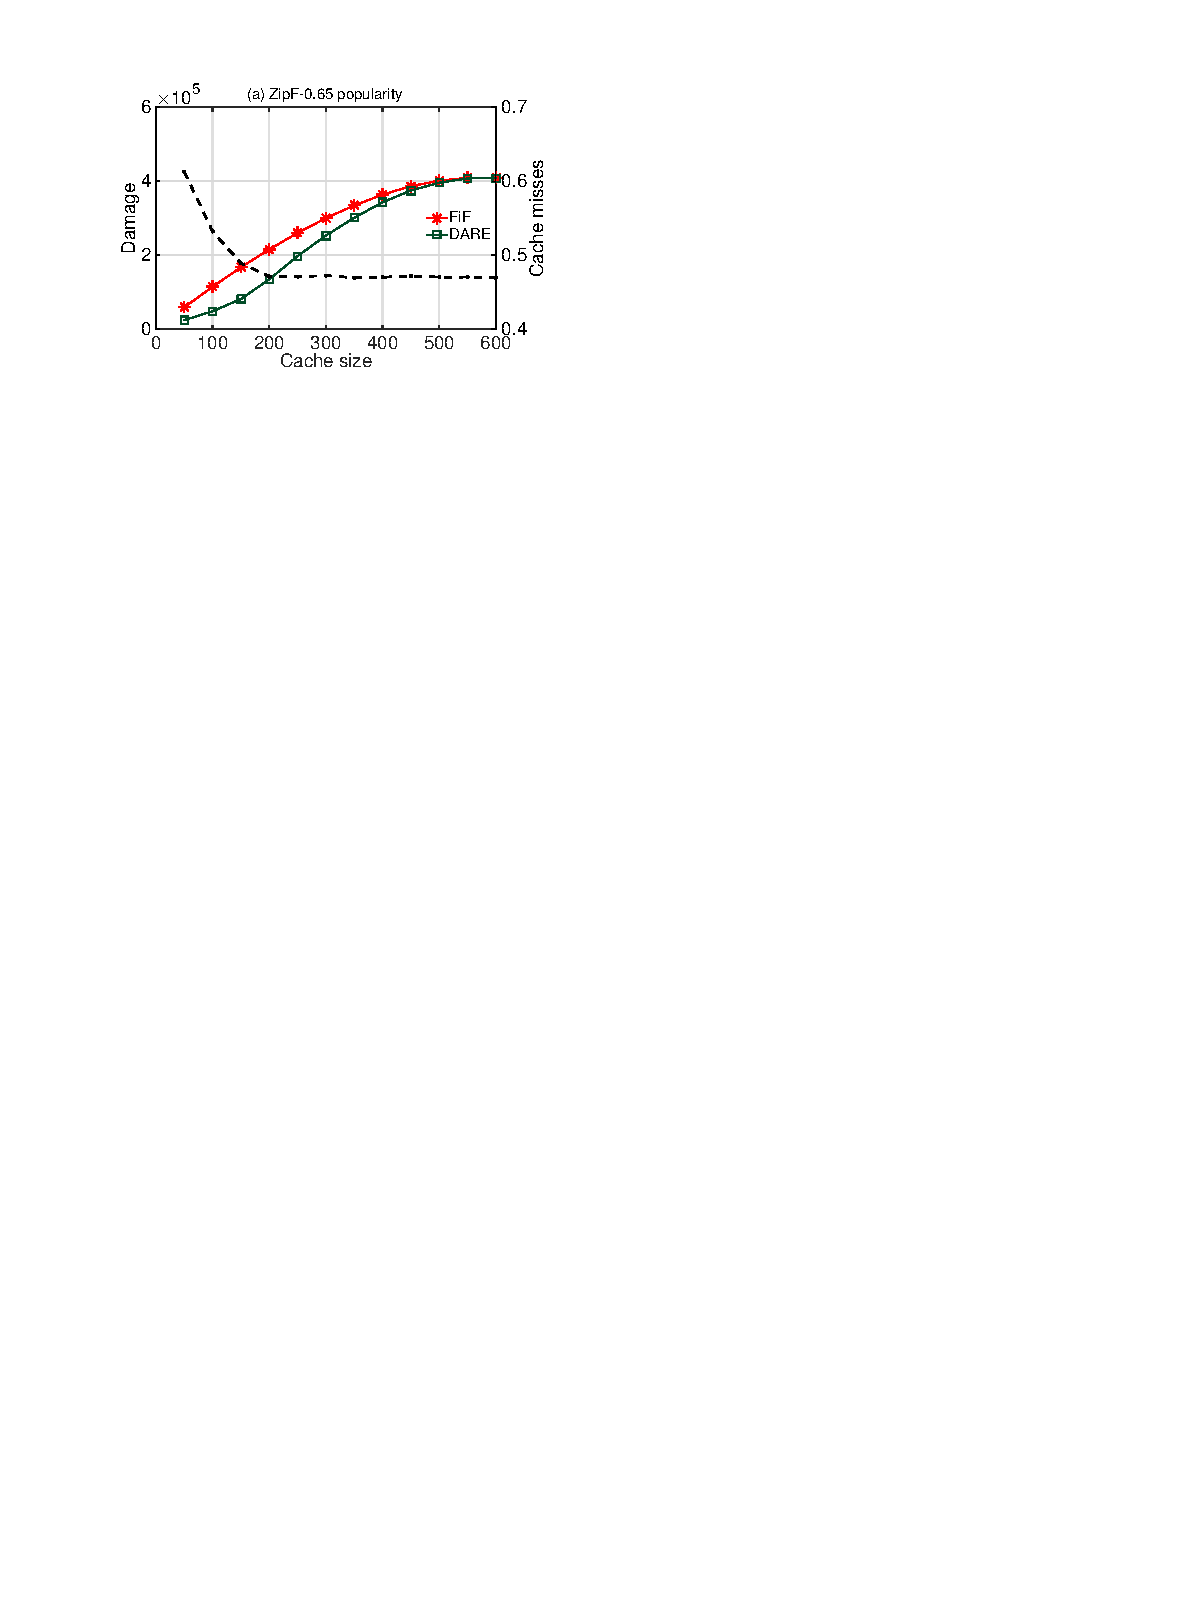
\includegraphics[width=0.45\textwidth]{figures/pic-pdf.pdf}}
  \caption{插入eps图像和pdf图像}
  \label{fig:pdfeps}
\end{figure}

\begin{lstlisting}[language={TeX}, caption={插入eps图像和pdf图像}][!htp]
\begin{figure}
  \centering
  \subfigure[EPS Figure]{
    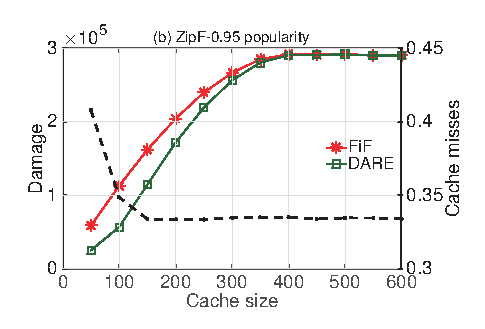
\includegraphics[width=0.45\textwidth]{figures/pic-eps}}
  \subfigure[PDF Figure]{
    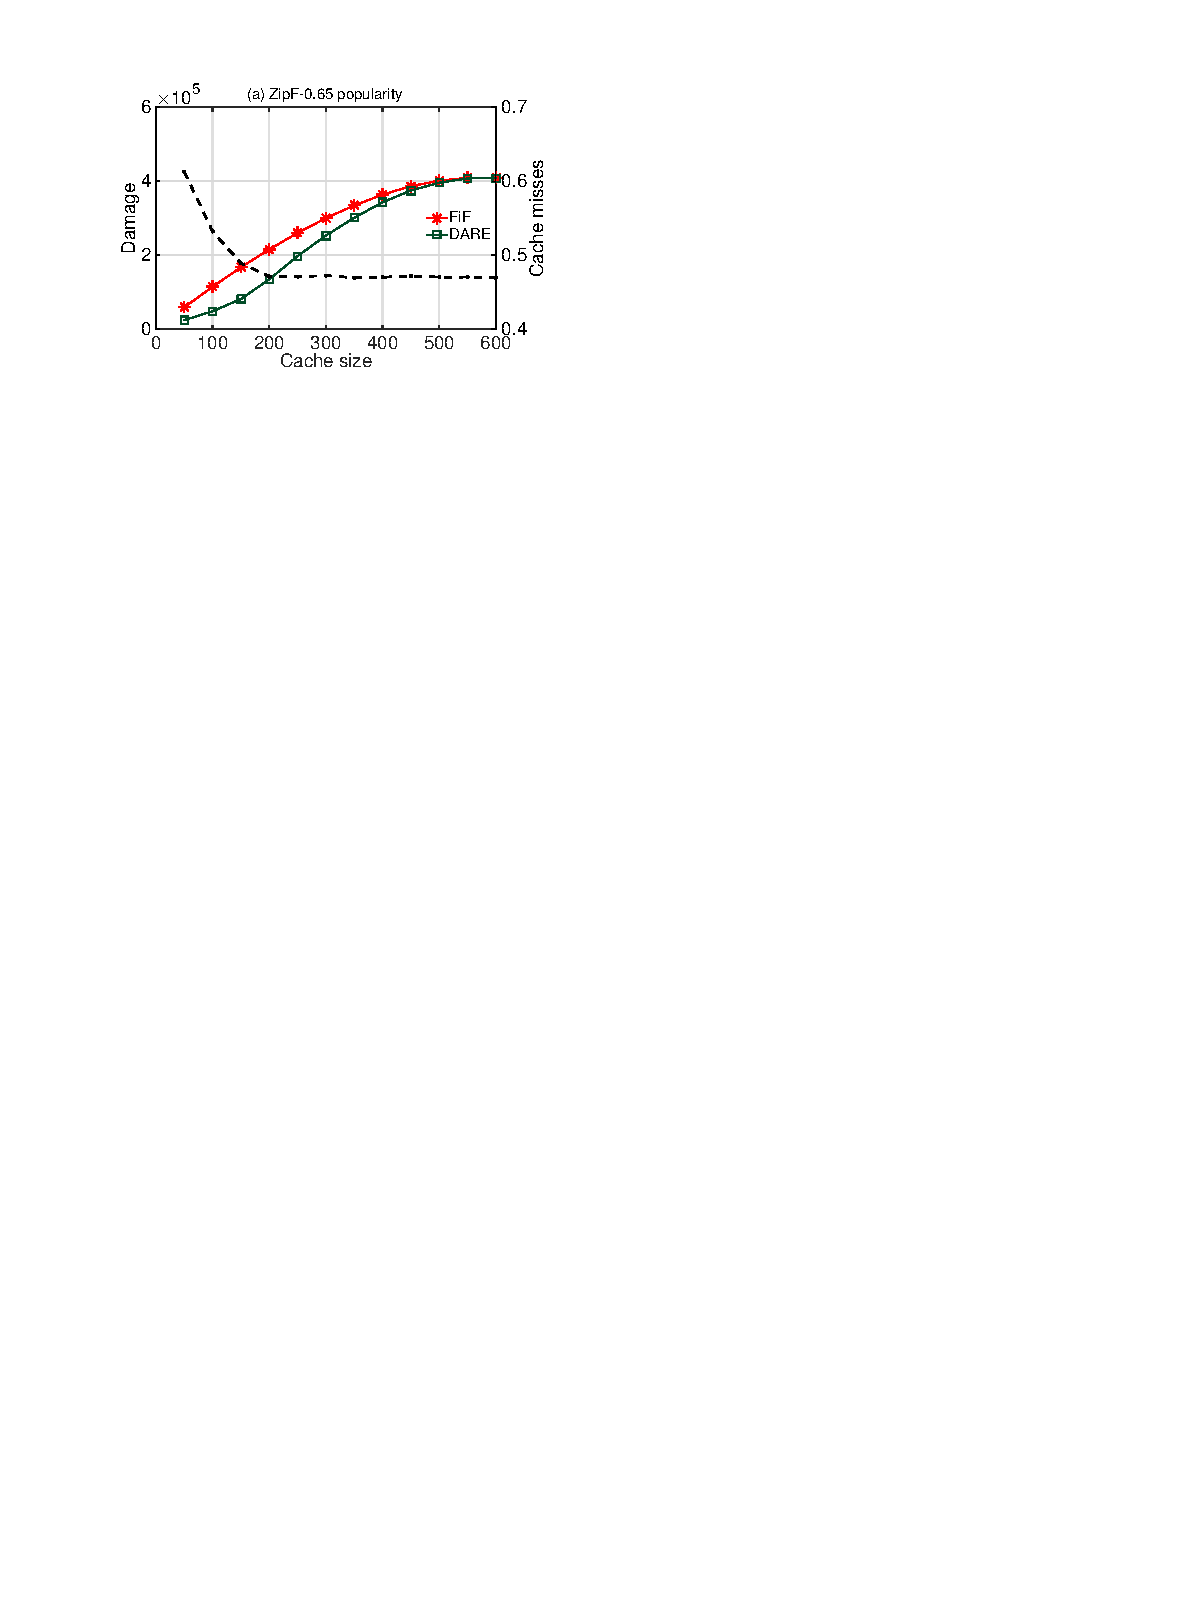
\includegraphics[width=0.45\textwidth]{figures/pic-pdf.pdf}}
  \caption{插入eps图像和pdf图像}
\end{figure}
\end{lstlisting}

更多关于~\LaTeX~ 插图的例子可以参考《~\LaTeX~插图指南》。

\subsection{长标题的换行}
\label{sec:longcaption}

图\ref{fig:longcaptionbad}和图\ref{fig:longcaptiongood}都有比较长图标题,通过对比发现,图\ref{fig:longcaptiongood}的换行效果更好一些。
其中使用了minipage环境来限制整个浮动题的宽度。

\begin{figure}[!htp]
 \centering
 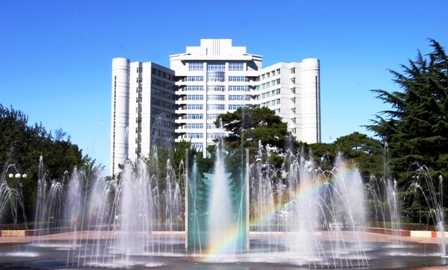
\includegraphics[width=10cm]{figures/pic1}
 \caption{BIT是我国历史最悠久的高等学府之一,是教育部直属、工信部共建的全国重点大学,985,211}
 \label{fig:longcaptionbad}
\end{figure}

\begin{figure}[!hbp]
  \centering
  \begin{minipage}[b]{0.6\textwidth}
  \captionstyle{\centering}
  \centering
  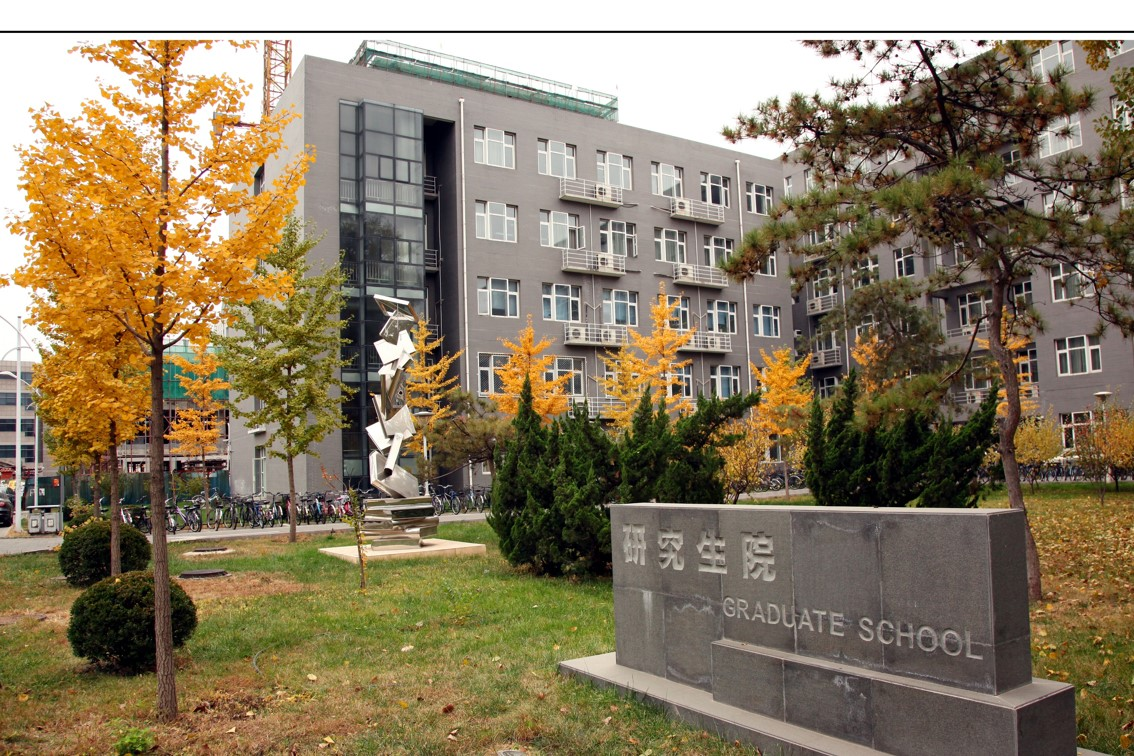
\includegraphics[width=10cm]{figures/pic2}
  \caption{BIT是我国历史最悠久的高等学府之一,是教育部直属、工信部共建的全国重点大学,985,211}
  \label{fig:longcaptiongood}
   \end{minipage}     
\end{figure}

\begin{lstlisting}[language={TeX}, caption={长标题的换行}]
\begin{figure}[!htp]
 \centering
 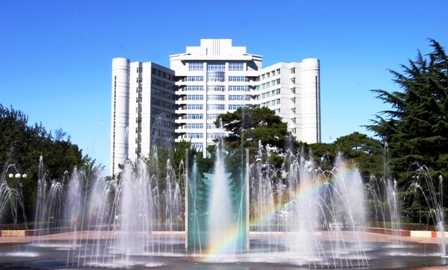
\includegraphics[width=10cm]{figures/pic1}
 \caption{BIT是我国历史最悠久的高等学府之一,是教育部直属、工信部共建的全国重点大学,985,211}
 \label{fig:longcaptionbad}
\end{figure}

\begin{figure}[!hbp]
  \centering
  \begin{minipage}[b]{0.6\textwidth}
  \captionstyle{\centering}
  \centering
  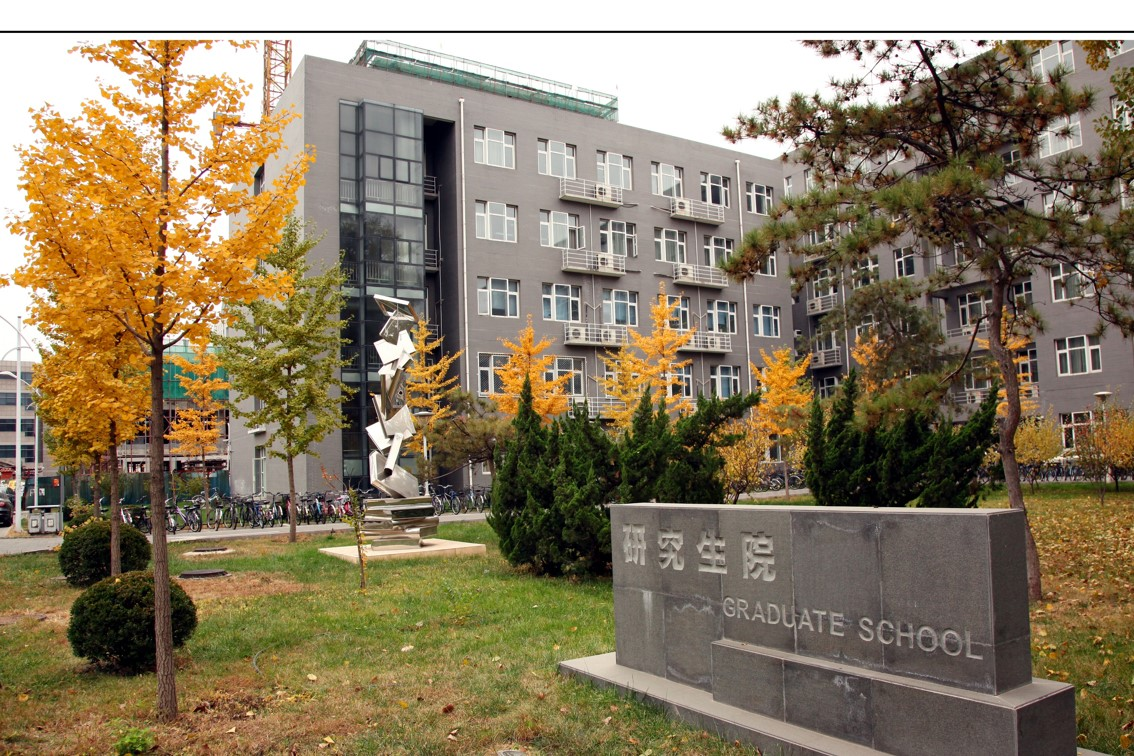
\includegraphics[width=10cm]{figures/pic2}
  \caption{BIT是我国历史最悠久的高等学府之一,是教育部直属、工信部共建的全国重点大学,985,211}
  \label{fig:longcaptiongood}
   \end{minipage}     
\end{figure}
\end{lstlisting}
  
\section{表格的例子}
\label{sec:tab}

表格的定义和引用已经在第~\ref{sec:refofFigAndTab}节中介绍,表格内容包含在\textbackslash begin\{table\}和\textbackslash end\{table\}之间。这里给出一些表格的例子。

\begin{table}[htb]               % no placement specified: defaults to here, top, bottom, page
\centering
 \begin{center}
  \caption{Physical meaning of parameters in L-B model.}
  \label{tab:LB-parameters}
  \begin{tabular}{cl}
      \toprule
       Parameters & Physical meaning       \\
      \midrule   % \hline
       $C_{L\alpha}$ & Lift curve slope \\
       $a_{1}$ & Controls the shape of the stall curve \\
       $\alpha^{\star}$ & The break point at which $X=0.5$ \\
       $\tau_{1}$ & Represents the tendency of the model to track the static curve \\
       $\tau_{2}$ & Gives the model lift overshoot \\
      \bottomrule
  \end{tabular}
 \end{center}
\end{table}

\begin{lstlisting}[language={TeX}, caption={插入表格}]
\begin{table}[htb]
\centering
 \begin{center}
  \caption{Physical meaning of parameters in L-B model.}
  \begin{tabular}{cl}
      \toprule
       Parameters & Physical meaning       \\
      \midrule 
       $C_{L\alpha}$ & Lift curve slope \\
       $a_{1}$ & Controls the shape of the stall curve \\
       $\alpha^{\star}$ & The break point at which $X=0.5$ \\
       $\tau_{1}$ & Represents the tendency of the model to track the static curve \\
       $\tau_{2}$ & Gives the model lift overshoot \\
      \bottomrule
  \end{tabular}
 \end{center}
\end{table}
\end{lstlisting}

再给出一些表格的例子,如表\ref{tab:firstone}所示。

\begin{table}[!htp]
  \centering
  \bicaption[tab:firstone]{指向一个表格的表目录索引}{一个颇为标准的三线表格\footnotemark[1]}{Table}{A Table}
  \begin{tabular}{@{}llr@{}} \toprule
    \multicolumn{2}{c}{Item} \\ \cmidrule(r){1-2}
    Animal & Description & Price (\$)\\ \midrule
    Gnat & per gram & 13.65 \\
    & each & 0.01 \\
    Gnu & stuffed & 92.50 \\
    Emu & stuffed & 33.33 \\
    Armadillo & frozen & 8.99 \\ \bottomrule
  \end{tabular}
\end{table}

下面一个是一个更复杂的表格,用threeparttable实现带有脚注的表格,如表\ref{tab:footnote}。

\begin{table}[!htp]
  \bicaption[tab:footnote]{出现在表目录的标题}{一个带有脚注的表格的例子}{Table}{A Table with footnotes}
  \centering
  \begin{threeparttable}[b]
     \begin{tabular}{ccd{4}cccc}
      \toprule
      \multirow{2}{6mm}{total}&\multicolumn{2}{c}{20\tnote{1}} & \multicolumn{2}{c}{40} &  \multicolumn{2}{c}{60}\\
      \cmidrule(lr){2-3}\cmidrule(lr){4-5}\cmidrule(lr){6-7}
      &www & k & www & k & www & k \\
      \midrule
      &$\underset{(2.12)}{4.22}$ & 120.0140\tnote{2} & 333.15 & 0.0411 & 444.99 & 0.1387 \\
      &168.6123 & 10.86 & 255.37 & 0.0353 & 376.14 & 0.1058 \\
      &6.761    & 0.007 & 235.37 & 0.0267 & 348.66 & 0.1010 \\
      \bottomrule
    \end{tabular}
    \begin{tablenotes}
    \item [1] the first note.% or \item [a]
    \item [2] the second note.% or \item [b]
    \end{tablenotes}
  \end{threeparttable}
\end{table}



\section{参考文献管理}

\subsection{将参考文献的内容与表现分离}

这个论文模板使用BibTeX处理参考文献,
BibTeX是最为流行的参考文献数据组织格式之一。它的出现让我们摆脱手写参考文献条目
的麻烦。
当然,使用者也可以手动编参考文献item,直接插入文档中。但是,有BibTeX帮助,处理起参考文献更为简单。我们还可以通过参考文献格式的支持,让同一份BibTeX数据库生成不同格式的参考文
献列表。

参考文献的``内容''就是reference文件夹下的chap\textit{xx}.bib,参考文献的元数据(名称、作者、出处等)以一定的格式保存在这些纯文本文件中。
.bib文件也可以理解为参考文献的``数据库'',正文中所有引用的参考文件条目都会从这些文件中``析出''。
控制参考文献条目``表现形式''(格式)的是.bst文件。.bst文件定义了参考文献风格,使用不同的参考文献风格能将同一个参考文献条目输出成不同的格式。
当然,一个文档只能使用一个参考文献风格。
按照学校要求,本模板使用的是国标GBT7714风格的参考文献。

BibTeX的工作过程是这样的:
BibTeX读取.aux(第一次运行latex得到的)查看参考文献条目,
然后到.bib中找相关条目的信息,
最后根据.bst的格式要求将参考文献条目格式化输出,写到.bbl文件中。
在运行latex将.bbl插入文档之前,可以用文本编辑器打开它,做一些小的修改。
.bbl的格式和你自己手动写item很相似,它已经被赋予了一定的``表现形式''。

.bib数据库中的参考文献条目可以手动编写,也可以在google的学术搜索中找到。
各大数据库也支持将参考文献信息导出为.bib,省时省力。
以Google学术搜索为例:在``学术搜索设置''中,将``文献管理软件''设为``显示导入BibTeX''的连接,保存退出。
然后学术搜索找到文献下会有``导出到BibTeX''连接,点击后Firefox会打开新的标签页,出现类似代码\ref{googlescholar}所示的内容
\footnote{展示这些.bib条目使用了listings宏包,因为listings宏包协调中文的能力很糟糕,所以读者在查看模板的这部分源代码时会看到一些非常麻烦的东西。并且,直接将源代码的这部分内容复制到.bib中可能还会出错。建议这部分内容留意PDF就足够了。}。
请注意,这个条目离``规范''还有一些距离。

  \begin{lstlisting}[caption={从Google Scholar找到的,但并不规范的.bib条目}, label=googlescholar, float, escapeinside="", numbers=none]
    @phdthesis{" 白2008信用风险传染模型和信用衍生品的定价 ",
      title={{" 信用风险传染模型和信用衍生品的定价 "}},
      author={" 白云芬 "},
      year={2008},
      school={" 上海交通大学 "}
    } 
  \end{lstlisting}

  上面的.bib条目的``名字''\cndash{}``白2008信用风险传染模型和信用衍生品的定价'',包含~ASCII~以外的字符,BibTeX无法处理;
  条目还缺少了address域,这样编译出来的结果会出现``地址不详'';
  并且,条目还缺少language域,BibTeX需要language域来判断是否是中文参考文献。
  将上面的条目修正(改英文名、增加address和language域),复制到本地的.bib文件中就可以了。
  显然,这里描述的是参考文献的内容,而不是表现形式。

  \begin{lstlisting}[caption={一个符合规范的.bib条目}, label=itemok, float, escapeinside="", numbers=none]
@article{ Jiang2005Size,
  title={ 形状记忆聚合物研究现状与发展 },
  author={ 姜敏 and 彭少贤 and 郦华兴 },
  journal={ 现代塑料加工应用 },
  volume={17},
  number={2},
  pages={53-56},
  year={2005},
}
  \end{lstlisting}

由于中英文参考文献处理起来有差异,所以需要在参考文献中标注是否是中文文献。
确切地说,BibTeX并不具有区分中英文参考文献的``智能'',这种智慧的来源是.bst文——它定义了处理参考文献的规则。
GBT7714-2005NLang.bst中规定:.bib中的条目,如果条目的``language''域非空,就被认为是中文文献,否则被认为是英文文献。
例如,刚才的文献,就会被认为是中文参考文献,采取一些针对中文的处理方式。

最后,这个条目被bibtex处理后,赋予了一定的``表现形式'',在.bbl文件中以下面的样子出现。
还可以对它进行小的修改,但较为麻烦。然后再次运行latex之后,它将被插入到文档中。

\begin{lstlisting}[caption={.bbl中被格式化之后的条目}, escapeinside="", numbers=none]
\bibitem{Jiang2005Size}
	姜敏, 彭少贤, 郦华兴.
	形状记忆聚合物研究现状与发展~[J].
	现代塑料加工应用, 2005, 17~(2):  53--56.
\end{lstlisting}

.bst文件书写起来非常繁杂\footnote{可以参考《Tame The BeaST》。},书写符合GBT7714标准的.bst文件更是一项浩大的工程。
因此,当大家为漂亮、标准的参考文献列表感到满意时,应该对
GBT7714-2005NLang.bst的作者充满谢意。{\color{red} 同时强调一下,由于学校
  规定参考文献采用5号字体,所以在使用此规范时,需要在前面加上字号限制:
\begin{lstlisting}
{
\zihao{5}
\bibliography{reference/chap1,reference/figures/chap2}
}
\end{lstlisting}}

另外,.bib是“参考文献的内容”,而控制参考文献表现(格式)的是.bst文件,本模板附带的是GBT7714-2005NLang.bst。

\subsection{在正文中引用参考文献}

参考文献可以分章节管理,只需要在主文件中的参考文献中都包含进去就可以,如\verb+\bibliography{chap1,figures/chap2,...}+。

正文中引用参考文献时\citep{Jiang2005Size},用\verb+\upcite{key1,key2,key3...}+可以产生“上标引用的参考文献”,
如\upcite{Meta_CN,chen2007act,DPMG}。
使用\verb+\cite{key1,key2,key3...}+则可以产生水平引用的参考文献,例如\cite{JohnD,zhubajie,IEEE-1363}。
请看下面的例子,将会穿插使用水平的和上标的参考文献:关于书的\cite{Meta_CN,JohnD,IEEE-1363},关于期刊的\upcite{chen2007act,chen2007ewi},
会议论文\cite{DPMG,kocher99,cnproceed},
硕士学位论文\cite{zhubajie,metamori2004},博士学位论文\upcite{shaheshang,FistSystem01,bai2008},标准文件\cite{IEEE-1363},技术报告\upcite{NPB2},电子文献\cite{xiaoyu2001, CHRISTINE1998}。

最后总结一些注意事项:
\begin{itemize}
\item  参考文献只有在正文中被引用了,才会在最后的参考文献列表中出现;
\item  参考文献``数据库文件''.bib是纯文本文件,请使用~UTF-8~编码,不要使用~GBK~编码;
\item  参考文献条目中通过~language~域是否为空判断是否是中文文献;
\item  参考文献条目同样有“内容”和“表现形式”之分,这种可控性是BibTeX带来的。
\end{itemize}


\section{用~listings~插入源代码}

这里给使用~listings~宏包插入源代码的例子,这里是一段C代码。另外,listings宏包可以实现各种复杂、漂亮的效果,想要进一步学习的同学,可以参考《The Listings Package》。

\begin{lstlisting}[language={C}, caption={一段C源代码}]
#include <stdio.h>
#include <unistd.h>
#include <sys/types.h>
#include <sys/wait.h>

int main() {
  pid_t pid;

  switch ((pid = fork())) {
  case -1:
    printf("fork failed\n");
    break;
  case 0:
    /* child calls exec */
    execl("/bin/ls", "ls", "-l", (char*)0);
    printf("execl failed\n");
    break;
  default:
    /* parent uses wait to suspend execution until child finishes */
    wait((int*)0);
    printf("is completed\n");
    break;
  }

  return 0;
}
\end{lstlisting}

再给一个插入MATLAB代码的例子。

\begin{lstlisting}[language={matlab}, caption={一段MATLAB源代码}]
function paper1
r=0.05;
n=100;
T=1;
X=1;
v0=0.8;
sigma=sqrt(0.08);
deltat=T/n;
for i=1:n
    t(i)=i*deltat;
    w(i)=random('norm',0,t(i),1);
end
for i=1:n
    alpha(i)=0.39;
end
for i=1:n
    temp=0;
    for k=1:i
        temp=temp+alpha(k);
    end
    B(i)=exp(r*t(i));
    BB(i)=B(i)*exp(temp*deltat);
    BBB(i)=exp(-r*(T-t(i)));
end
for i=1:n
    s0(i)=X*BBB(i);
    v(i)=v0*exp((r-0.5*sigma^2)*t(i)+sigma*w(i));
    for j=i+1:n
        D=X*BBB(j);
        d1=(log(v(i)/D)+(r+sigma^2/2)*(t(j)-t(i)))/(sigma*sqrt(t(j)-t(i)));
        d2=d1-(sigma*sqrt(t(j)-t(i)));
        ppp(i,j)=D*exp(-r*(t(j)-t(i)))*(1-cdf('normal',d2,0,1))-v(i)*(1-cdf('n
ormal',d1,0,1));
    end
end
for i=1:n
    s1(i)=0;
    for j=i+1:n
        s1(i)=s1(i)+BB(j)^(-1)*alpha(j)*deltat*(X*BBB(j)-B(j)/B(i)*ppp(i,j));
    end
    s2(i)=0;
    for j=1:n
        s2(i)=s2(i)+alpha(j);
    end
    s2(i)=X*exp(-r*T-s2(i)*deltat);
    s(i)=BB(i)*(s1(i)+s2(i));
end
plot(s)
hold on;
plot(s0);
\end{lstlisting}

%%==================================================
%% ch4.tex for BIT Master Thesis
%% modified by yang yating
%% version: 0.2
%% last update: Feb 16th, 2017
%%==================================================


\chapter{论文格式的调整}
\label{sec:thesisformat}

\textbf{一般的学生不需要进行论文格式的调整。原则上,使用最新版本的BIT-Thesis进行论文的编写即可生成符合学校毕业设计论文格式要求的论文。如果需要个性化修改,可根据此章的说明。
}

这个模板可支持``单面打印''和``双面打印''。你可以在~demo.tex~
中设定文档类的语句中进行相应修改:

单面打印
\begin{lstlisting}[language={TeX}]
\documentclass[oneside, master]{BIT-thesis-grd} %硕士
\documentclass[oneside, doctor]{BIT-thesis-grd} %博士
\end{lstlisting}

双面打印
\begin{lstlisting}[language={TeX}]
\documentclass[twoside, master]{BIT-thesis-grd} %硕士
\documentclass[twoside, doctor]{BIT-thesis-grd} %博士
\end{lstlisting}

关于页眉页脚,按照BIT要求:

页眉为``北京理工大学XX学位论文'',XX表示博士或
硕士,宋体、5号,居中排列;页眉从中文摘要开始标注,论文页眉奇偶页相同。页
码从第1章(绪论)开始按阿拉伯数字(1,2,3……)连续编排,之前的部分(中文摘
要、Abstract、目录等)用大写罗马数字(Ⅰ,Ⅱ,Ⅲ……)单独编排。

研究生院要求参考文献必须符合~GBT7714~风格。使用这个模板,结合BibTeX,可
以很方便地生成符合GB标准的参考文献列表。

具体的格式参见《北京理工大学博士、硕士学位论文撰写规范》格式要求。

论文模板主要在bit-master-thesis.cls文件中进行定义,现对其进行简单介绍。
\section{页面设置}
页边距设置如下:
\begin{lstlisting}[language={TeX}]
\usepackage[
paper=a4paper,
top=3.5cm,% 上 3.5cm
bottom=2.5cm,% 下 2.5cm
left=2.7cm,% 左 2.7cm
right=2.7cm,% 右 2.7cm
headheight=1.0cm,% 页眉 2.5cm
footskip=0.7cm% 页脚 1.8cm
]{geometry} % 页面设置
\end{lstlisting}

行距离设置,按照要求,应该为22榜,如下设置:
\begin{lstlisting}[language={[LaTeX]TeX}]
\RequirePackage{setspace}
\setstretch{1.523} 
\end{lstlisting}

\section{章节格式与目录}
严格按照规范,采用如下代码实现:
\begin{lstlisting}language={TeX}
%% 设置章节格式
\ctexset{chapter={
      name = {第,章},
      number = {\arabic{chapter}},
      format = {\bfseries \heiti \centering \zihao{3}},
      pagestyle = {BIT@headings},
      beforeskip = 16bp,
      afterskip = 28bp,
      fixskip = true,
  }
}
%% 设置一级章节格式
\ctexset{section={
  format={\raggedright \bfseries \heiti \zihao{4}},
  beforeskip = 28bp plus 1ex minus .2ex,
  afterskip = 24bp plus .2ex,
  fixskip = true,
  }
}

% 设置二级标题格式
%黑体小四加粗顶左,单倍行距,序号与题目间空一个汉字符
\ctexset{subsection={
   format = {\bfseries \heiti \raggedright \zihao{-4}},
   beforeskip =28bp plus 1ex minus .2ex,
   afterskip = 24bp plus .2ex,
   fixskip = true,
   }
}
% 设置三节标题格式:黑体小四居左书写,单倍行距,序号与题目间空一个汉字符
\ctexset{subsubsection={
      format={\heiti \raggedright \zihao{-4}},
      beforeskip=28bp plus 1ex minus .2ex,
      afterskip=24bp plus .2ex,
      fixskip=true,
  }
}
%% 用\textsf{titletoc}设定目录格式。
\RequirePackage{titletoc}
\titlecontents{chapter}[0pt]{\vspace{0.25\baselineskip} \songti \zihao{4}}
    {\thecontentslabel\quad}{}
    {\hspace{.5em}\titlerule*{.}\contentspage}
\titlecontents{section}[2em]{\songti \zihao{-4}}
    {\thecontentslabel\quad}{}
    {\hspace{.5em}\titlerule*{.}\contentspage}
\titlecontents{subsection}[4em]{\songti \zihao{-4}}
    {\thecontentslabel\quad}{}
    {\hspace{.5em}\titlerule*{.}\contentspage}
    
\end{lstlisting}

\section{封面设计}
这里我们为封面设计提供了众多命令,以中文封面为例:
\begin{lstlisting}language={TeX}
%%%%中文标题页的可用命令
\newcommand\classification[1]{\def\BIT@value@classification{#1}}
\newcommand\studentnumber[1]{\def\BIT@value@studentnumber{#1}}
\newcommand\confidential[1]{\def\BIT@value@confidential{#1}}
\newcommand\UDC[1]{\def\BIT@value@UDC{#1}}
\newcommand\serialnumber[1]{\def\BIT@value@serialnumber{#1}}
\newcommand\school[1]{\def\BIT@value@school{#1}}
\newcommand\degree[1]{\def\BIT@value@degree{#1}}
\renewcommand\title[2][\BIT@value@title]{%
  \def\BIT@value@title{#2}
  \def\BIT@value@titlemark{\MakeUppercase{#1}}}
\renewcommand\vtitle[1]{\def\BIT@value@vtitle{#1}}
\renewcommand\author[1]{\def\BIT@value@author{#1}}
\newcommand\advisor[1]{\def\BIT@value@advisor{#1}}
\newcommand\advisorinstitute[1]{\def\BIT@value@advisorinstitute{#1}}
\newcommand\major[1]{\def\BIT@value@major{#1}}
\newcommand\submitdate[1]{\def\BIT@value@submitdate{#1}}
\newcommand\defenddate[1]{\def\BIT@value@defenddate{#1}}
\newcommand\institute[1]{\def\BIT@value@institute{#1}}
\newcommand\chairman[1]{\def\BIT@value@chairman{#1}}

\end{lstlisting}

使用这些命令,即可在主控文件中设置自己的封面,例如本文档在demo.tex中如下
设置:
\begin{lstlisting}[language={TeX}]
\classification{****.*}
\UDC{***}
\title{****}
\author{****}
\institute{****}
\advisor{****}
\chairman{****}
\degree{****}
\major{****}
\school{ 北京理工大学}
\defenddate{****}
\end{lstlisting}

这些变量设置好之后,\\使用\verb+\maketitle+产生封面的第一页;\\使用
\verb+\makeInfo+产生中文信息页;\\使用
\verb+\makeEnglishInfo+产生英文信息页;\\使用\verb+\makeVerticalTitle+产
生竖着排放的标题页;\\使用\verb+\makeDeclareOriginal+产生声明页。

%%%%==================================================
%% ch5.tex for BIT Master Thesis
%% modified by yang yating
%% version: 0.2
%% last update: Feb 16th, 2017
%%==================================================

% \bibliographystyle{sjtu2} %[此处用于每章都生产参考文献]

\chapter{存在的问题}
\label{chap:needsomehelp}

由于时间非常仓促,这个模板肯定存在不少问题

。。。





%%==================================================
%% conclusion.tex for BIT Master Thesis
%% modified by yang yating
%% version: 0.1
%% last update: Dec 25th, 2016
%%==================================================


\chapter*{总结\markboth{总结}{}}
\addcontentsline{toc}{chapter}{总结}

本文采用……。{\color{blue}(结论作为学位论文正文的最后部分单独排写,但不加章号。结论是对整个论文主要结果的总结。在结论中应明确指出本研究的创新点,对其应用前景和社会、经济价值等加以预测和评价,并指出今后进一步在本研究方向进行研究工作的展望与设想。结论部分的撰写应简明扼要,突出创新性。)本文采用……。(结论作为学位论文正文的最后部分单独排写,但不加章号。结论是对整个论文主要结果的总结。在结论中应明确指出本研究的创新点,对其应用前景和社会、经济价值等加以预测和评价,并指出今后进一步在本研究方向进行研究工作的展望与设想。结论部分的撰写应简明扼要,突出创新性。)}
 %% 全文总结

% 参考文献
% 使用 BibTeX
% 包含参考文献文件.bib
{
\zihao{5}
\bibliography{reference/chap1,reference/chap2} %多个章节的参考文献
%\bibliography{reference/chap1}
}

%%%%%%%%%%%%%%%%%%%%%%%%%%%%%%
%% 附录(章节编号重新计算,使用字母进行编号)
%%%%%%%%%%%%%%%%%%%%%%%%%%%%%%

%处理章节编号
\appendix

%%==================================================
%% app1-content.tex for BIT Master Thesis
%% modified by yang yating
%% version: 0.2
%% last update: Feb 16th, 2017
%%==================================================
\chapter{北京理工大学博士、硕士学位论文内容要求}
\label{app:format}
《北京理工大学博士、硕士学位论文撰写规范》是参照国家标准GB7713-87《科学技术报告、学位论文和学术论文的编写格式》(GB77B-87),并结合我校具体情况制定的。

\section{封面}
封面是学位论文的外表,起提供信息和保护的作用。北京理工大学学位论文封面撰写要求如下:

\begin{enumerate}
\item 密级:必要时置于封面右上角,并按照国家规定进行标记。
\item 种类:博士或硕士学位论文。
\item 题目:应简明扼要地概括和反映出论文的核心内容,一般不宜超过25字。
\item 作者:位于论文题目正下方。
\item 时间:xxxx年xx月。
\end{enumerate}

\section{题名页}
\subsection{中文题名页}
题名页是对学位论文进行著录的依据。题名页自上而下的排列顺序为:中图分类号、UDC分类号、论文题目、作者姓名、学院名称、指导教师、答辩委员会主席、申请学位级别、学科专业、学位授予单位以及论文答辩日期等信息。

\begin{enumerate}
\item 分类号:必须在题名页左上角注明分类号,便于信息查询和交流。一般应注明《中国图书馆分类法》的分类号,同时注明《国际十进分类法UDC》的分类号。《中国图书馆分类法》分类号的选择通常是查阅最新版的《中国图书馆分类法》。国际十进分类法是最早的多语种分类法,在全世界得到了广泛的使用。国际十进分类号简表请参见UDC联盟网站http://www.udcc.org/outline/outline.htm。
\item 论文题目:中文题目同封面一致。
\item 作者姓名:位于论文题目正下方。
\item 学院名称:填写所属学院的全名。
\item 指导教师:填写指导教师的姓名、职称。指导教师的署名应以研究生院批准备案的为准,一般只能写一名指导教师,如有经研究生院批准的副指导教师或联合指导教师,可增写一名指导教师。
\item 答辩委员会主席:填写答辩委员会主席的姓名、职称。
\item 申请学位级别:填写“学科门类+学位级别”,如工学博士、理学硕士等;如申请专业学位,填写“类别+学位级别”,如工程硕士、工商管理硕士等。
\item 学科专业:学科专业名称参照国务院学位委员会颁布的《授予博士、硕士学位和培养研究生的学科、专业目录》填写,工程硕士填写工程领域。
\item 授予学位单位:北京理工大学
\item 论文答辩日期:xxxx年xx月xx日
\end{enumerate}

\subsection{英文题名页}
英文题名页包括英文题目、作者姓名、指导教师、学位授予单位及答辩日期。
英文题目是中文题目的直译,一般不超过15个实词。

\section{版权使用授权及研究成果声明}
作者和导师须亲笔签署版权使用授权及研究成果声明。

\section{摘要}
摘要是一篇具有独立性和完整性的短文,应概括而扼要地反映出本论文的主要内容。包括研究目的、研究方法、研究结果和结论等,特别要突出研究结果和结论。中文摘要力求语言精炼准确,硕士学位论文摘要建议500 $\sim$ 800字,博士学位论文建议1000 $\sim$ 1200字。摘要中不可出现参考文献、图、表、化学结构式、非公知公用的符号和术语。英文摘要与中文摘要的内容应一致。

\section{关键词}
关键词是为了便于文献索引和检索而从论文中选取出来用以表示全文主题内容信息的单词或术语,在摘要内容后另起一行标明。一般选3~8个单词或专业术语,之间用空格分开,且中英文关键词必须对应。

\section{目录}
目录由论文的章、节、附录等的序号、名称和页码组成,另页排在摘要之后,一般分为二级或三级。目录中应包括绪论(或引言)、论文主体、附录、参考文献、攻读学位期间取得的成果等。

\section{插图和附表}
如论文中图表较多,可以分别列出清单置于目录页之后。图的清单应有序号、图题和页码。表的清单应有序号、表题和页码。

\section{注释表}
如果论文中使用了大量的符号、标志、缩略词、首字母缩写、专门计量单位、自定义名词和术语等,应编写成注释说明汇集表。若上述符号使用数量不多,可以不设此部分,但必须在论文中初次出现时加以说明。

\section{正文}
正文包括绪论、论文具体研究内容及结论部分。
博士学位论文:一般为6~10万字,其中绪论要求为1万字左右。
硕士学位论文:一般为3~5万字,其中绪论要求为0.5万字左右。

\subsection{绪论}
绪论一般作为第1章。绪论应包括本研究课题的学术背景及其理论与实际意义;本领域的国内外研究进展及成果、存在的不足或有待深入研究的问题;本研究课题的来源及主要研究内容等。

\subsection{具体研究内容}
具体研究内容是学位论文的主要部分,是研究结果及其依据的具体表述,是研究能力的集中体现,一般应包括第2章、第3章至结论前一章。具体研究内容应该结构合理,层次清楚,重点突出,文字简练、通顺。可包括以下各方面:研究对象、研究方法、仪器设备、材料原料、实验和观测结果、理论推导、计算方法和编程原理、数据资料和经过加工整理的图表、理论分析、形成的论点和导出的结论等。
具体研究内容各章后可有一节“本章小结”(必要时)。

\subsection{结论}
结论作为学位论文正文的最后部分单独排写,但不加章号。
结论是对整个论文主要结果的总结。在结论中应明确指出本研究的创新点,对其应用前景和社会、经济价值等加以预测和评价,并指出今后进一步在本研究方向进行研究工作的展望与设想。结论部分的撰写应简明扼要,突出创新性。


\section{参考文献}
为了反映论文的科学依据和作者尊重他人研究成果的严肃态度以及向读者提供有关信息的出处,应列出参考文献表。参考文献表中应列出限于作者直接阅读过的、最主要的、发表在正式出版物上的文献。私人通信和未公开发表的资料,一般不宜列入参考文献,可紧跟在引用的内容之后注释或标注在当页的下方。

\section{附录}
有些材料编入文章主体会有损于编排的条理性和逻辑性,或有碍于文章结构的紧凑和突出主题思想等,这些材料可作为附录另页排在参考文献之后,也可以单编成册。下列内容可作为附录:

\begin{enumerate}
\item 为了整篇论文材料的完整,但编入正文有损于编排的条理性和逻辑性的材料,这一类材料包括比正文更为详尽的信息、研究方法和技术等更深入的叙述,以及建议可阅读的参考文献题录和对了解正文内容有用的补充信息等;
\item 由于篇幅过大或取材的复制资料不便于编入正文的材料;
\item 不便于编入正文的罕见珍贵资料;
\item 一般读者无须阅读,但对本专业同行有参考价值的资料;
\item 某些重要的原始数据、推导、计算程序、框图、结构图、注释、统计表、计算机打印输出件等。
\end{enumerate}

附录的序号用A,B,C……系列,如附录A,附录B,……。附录中的公式、图和表的编号分别用各自的附录序号后标1,2,3……系列来表示,如A1,A2,……系列;图A1,图A2,……系列;表A1,表A2,…系列。每个附录应有标题。

\section{攻读学位期间发表的论文与研究成果清单}
应列出攻读学位期间发表的与学位论文内容相关的学术论文和研究成果,按发表的时间顺序列出,研究成果可以是在学期间参加的研究项目、获得专利、获奖情况等

\section{致谢}
致谢是对下列方面致谢:资助和支持者;协助完成研究工作和提供便利条件者;在研究工作中提出建议和提供帮助者;给予转载和引用权的资料、图片、文献、研究思想和设想的所有者;其他应感谢者。致谢语言要诚恳、恰当、简短。

\section{作者简介}
硕士学位论文不必提供作者简介。

博士学位论文应该提供作者简介,主要包括:姓名、性别、出生年月、民族、出生地;简要学历、工作经历(职务);攻读学位期间取得的其他研究成果或奖励。


%%==================================================
%% app2-material.tex for BIT Master Thesis
%% modified by yang yating
%% version: 0.2
%% last update: April 16th, 2017
%%==================================================
\chapter{学习资料}
\label{chap:material}

建议的学习资料已存在github仓库中,见\href{https://github.com/BIT-thesis/LaTex-template/tree/master/LaTex%E5%AD%A6%E4%B9%A0%E8%B5%84%E6%96%99}{LaTex学习资料}。

\begin{itemize}
\item C\TeX 常见问题合集
\item \LaTeX 插图指南
\item Math Mode
\item 一份不太简短的~\LaTeXe{}~介绍

\end{itemize}

\LaTex 除了可以用于写出规范的学位论文,还可用于写SCI等期刊论文。

\begin{itemize}
\item \href{http://www.ctan.org/tex-archive/macros/latex/contrib/IEEEtran/}{IEEE­论文模板}

\end{itemize} % 更新记录
%%==================================================
%% app2-log.tex for BIT Master Thesis
%% modified by yang yating
%% version: 0.2
%% last update: Feb 16th, 2017
%%==================================================
\chapter{模板更新记录}
\label{chap:updatelog}
\begin{itemize}
\item \textbf{2017年2月} 根据网上北理工 \LaTeX{} 论文模板“2012大眼小蚂蚁版”和“2016汪卫版”。本模板在此两个模板的基础上依据《北京理工大学博士、硕士学位论文撰写规范》进行修改和完善。

\item \textbf{2017年9月} 根据试用版反馈,修改BIT-Thesis v1.0。
\end{itemize}
 % 更新记录


%%%%%%%%%%%%%%%%%%%%%%%%%%%%%%
%% 文后(无章节编号)
%%%%%%%%%%%%%%%%%%%%%%%%%%%%%%
\backmatter 

% 发表文章目录
%%%==================================================
%% pub.tex  for BIT Master Thesis
%% modified by yang yating
%% version: 0.2
%% last update: Feb 16th, 2017
%%==================================================

\begin{publications}{99}

    \item\textsc{Chen H, Chan C~T}. {Acoustic cloaking in three dimensions using acoustic metamaterials}[J].
      Applied Physics Letters, 2007, 91:183518.

    \item\textsc{Chen H, Wu B~I, Zhang B}, et al. {Electromagnetic Wave Interactions with a Metamaterial Cloak}[J].
      Physical Review Letters, 2007, 99(6):63903.
    
\end{publications}

% 致谢
%%==================================================
%% thanks.tex  for BIT Master Thesis
%% modified by yang yating
%% version: 0.2
%% last update: April 27th, 2017
%%==================================================


\begin{thanks}


感谢计算机学院2016级研究生杨雅婷对模板的修改更新做了大量工作。本项目得到研究生院学位与学部办公室和学生事务中心的资助支持。

\end{thanks}


\end{document}
